\chapter{Introduction To Astrid}\label{chap:astrid}
 
%++++++++++++++++++++++++++++++++++++++++++++++++++++++++++++++++++++++++++++
\section{What Is Astrid?}

\gls{Astrid} is a single, unified workspace that incorporates a suite of applications 
that can be used with the \gls{GBT}. \gls{Astrid} provides a single interface from
which the observer can create, execute and monitor observations with the \gls{GBT}.
Some of the features of \gls{Astrid} are:

\begin{itemize}[leftmargin=*]
\item Executes \glsfirstplural{SB} to perform astronomical observations.
\item Provides a real time display of \gls{GBT} data
\item Provides the status of the \gls{GBT}.
\item Provides an area to edit \glspl{SB}. They may be edited offline and saved before
observing.
\item Allows a second observer to monitor observations in progress.
\end{itemize}

\gls{Astrid} brings together many applications into a single, unified \gls{GUI}.
Of particular note, \gls{Astrid} provides a single point of contact to all of
the \gls{MC} software by interpreting the Python code and function in \glspl{SB}.
The \gls{GBT} \gls{MC} systems can roughly be thought of as a group of programs
- one for each hardware device - and a master program, the Scan Coordinator.
The \gls{GUI} places each application into its own tab window.  Applications
available in \gls{Astrid} are:

\begin{description}
\item[Observation Management]\ \\
\gls{Astrid} interfaces with the Observing Management Application in order to
execute \glspl{SB}.  The \gls{Astrid} Edit Subtab (see \S~\ref{sec:editsubtab})
provides a windows-like text editor that features syntax highlighting for
Python code and allows \glspl{SB} to be edited, validated, copied, and saved.
\glspl{SB} may be queued and executed via the \gls{Astrid} Run Subtab
(see \S~\ref{sec:runsubtab}).

\item[Data Display]\ \\
\gls{Astrid} provides a real time data display by connecting to \gls{GFM}.
This allows the automatic processing of pointing and focus scans that can
immediately update the \gls{GBT} \gls{MC} system with the determined
corrections.  \gls{GFM} can show raw, uncalibrated continuum data as
a function of time (see Chapter~\ref{chap:datadisplay}).

\item[GBT Status]\ \\
\gls{Astrid} provides a screen that displays information on the real time
status of the \gls{GBT}. This provides meta--information such as the \gls{LST},
\gls{UTC}, observer, project ID, information on the antenna such as current
position, and information on the current scan and \gls{IF} setup
(see \S~\ref{sec:astridstatus}).
\end{description}

\newpage
%++++++++++++++++++++++++++++++++++++++++++++++++++++++++++++++++++++++++++++
\section{How To Start Astrid}\label{sec:startingastrid}
 
To start \gls{Astrid}, type {\tt astrid} from the command line on any Linux
computer in Green Bank. The first thing you will see is the \gls{Astrid}
\dq{splash screen} which is shown in Figure~\ref{fig:astridsplash}. The
\gls{Astrid} \gls{GUI} should appear on-screen after 10-20 seconds
(see Figure~\ref{fig:astridcomposition}).

\begin{minipage}[b]{0.36\linewidth}
\vspace{0pt}
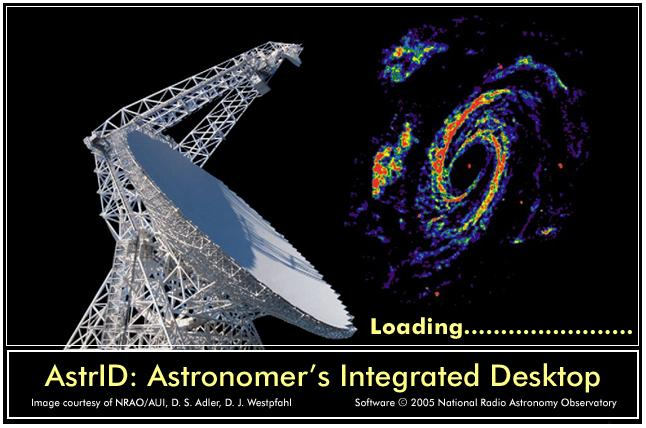
\includegraphics[width=\linewidth]{AstridSplash.jpg}
\captionof{figure}[Astrid splash screen]
{The \gls{Astrid} splash screen.
\label{fig:astridsplash}}
\end{minipage}
\hfill
\begin{minipage}[b]{0.43\linewidth}
\vspace{0pt}
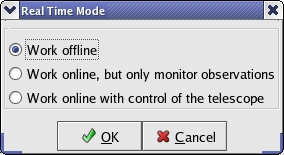
\includegraphics[width=\linewidth]{AstridMode.jpg}
\captionof{figure}[Astrid startup pop-up window]
{\gls{Astrid} startup pop-up window.
\label{fig:astridmode}}
\end{minipage}

\vspace{-5mm}

\subsection{Astrid Modes}\label{sec:astridmode}

\noindent On startup, \gls{Astrid} will automatically ask what mode to operate in via
the pop-up window shown in Figure~\ref{fig:astridmode}.  Once an initial mode has been
set it may be changed at any time by selecting {\tt Real Time Mode...} from the {\tt File}
drop-down menu (see \S~\ref{sec:dropdownmenus}).

{\bf Note} that observers should use {\tt File}$\rightarrow${\tt Real Time Mode...} to
relinquish control of the telescope immediately after their scheduled observing session.

\begin{table}[!h]
\begin{center}
\caption[Astrid online and offline modes]{\gls{Astrid} mode features}\label{table:astridmodes}
\begin{tabular}{lccccl}
\toprule
{\bf Mode}             & Edit \&         &  Validate      & Submit     & Observing & \multicolumn{1}{c}{Data}    \\
                       & Validate Syntax &  Configuration & \glspl{SB} &   Logs    & \multicolumn{1}{c}{Display} \\
\midrule
{\bf Offline}          & \checkmark      & Simulated      &            &           & Historical$^{(1)}$ \\
{\bf Online (monitor)} & \checkmark      & Simulated      &            &\checkmark & Real-time \\
{\bf Online (control)} & \checkmark      & Real$^{(2)}$    & \checkmark$^{(3)}$ &\checkmark & Real-time \\
\bottomrule
\end{tabular}
\footnotesize{
\begin{itemize}[itemsep=0pt]
\item[$(1)$] Previously acquired data should always be viewed \sq{offline}.
\item[$(2)$] Requested configurations are validated with respect to the actual
{\tt dev\_health.conf} file rather than\newline the simulated \sq{ideal} universal cabling file.
\item[$(3)$] Only permitted when you are \sq{in the gateway} (the \gls{GBT} operator has given you
security access).
\end{itemize}
}
\end{center}
\end{table}

\noindent The features available for each mode are listed in
table~\ref{table:astridmodes}.  Users should select the most appropriate
mode for their purposes:

\begin{itemize}[leftmargin=*]
\item {\bf Work offline}: Primarily used to create, edit and validate \glspl{SB}.
It is also the preferred method to look at previously obtained data in the Data
Display since online modes will continually refresh the display window with
near-real-time data.

\item {\bf Work online, but only monitor observations}: May be used to view what
is happening in the \gls{Astrid} observing logs and Data Display for the current
observations. You will not be able to submit \glspl{SB} or affect observing in any
manner.

\item {\bf Work online with control of the telescope}: Used to perform observations
with the \gls{GBT} by allowing the user to submit \glspl{SB}. Log information and
real-time data displays are also available in this mode.
{\bf Note that working online requires the \gls{GBT} operator to \dq{put you
in the gateway} (give you security access).}
\end{itemize}

\newpage

\section{Astrid GUI Composition}\label{sec:astridcomposition}

The \gls{Astrid} \gls{GUI} layout consists of several components shown in
Figure~\ref{fig:astridcomposition} and described in the following section.

\begin{figure}[!h]
\begin{center}
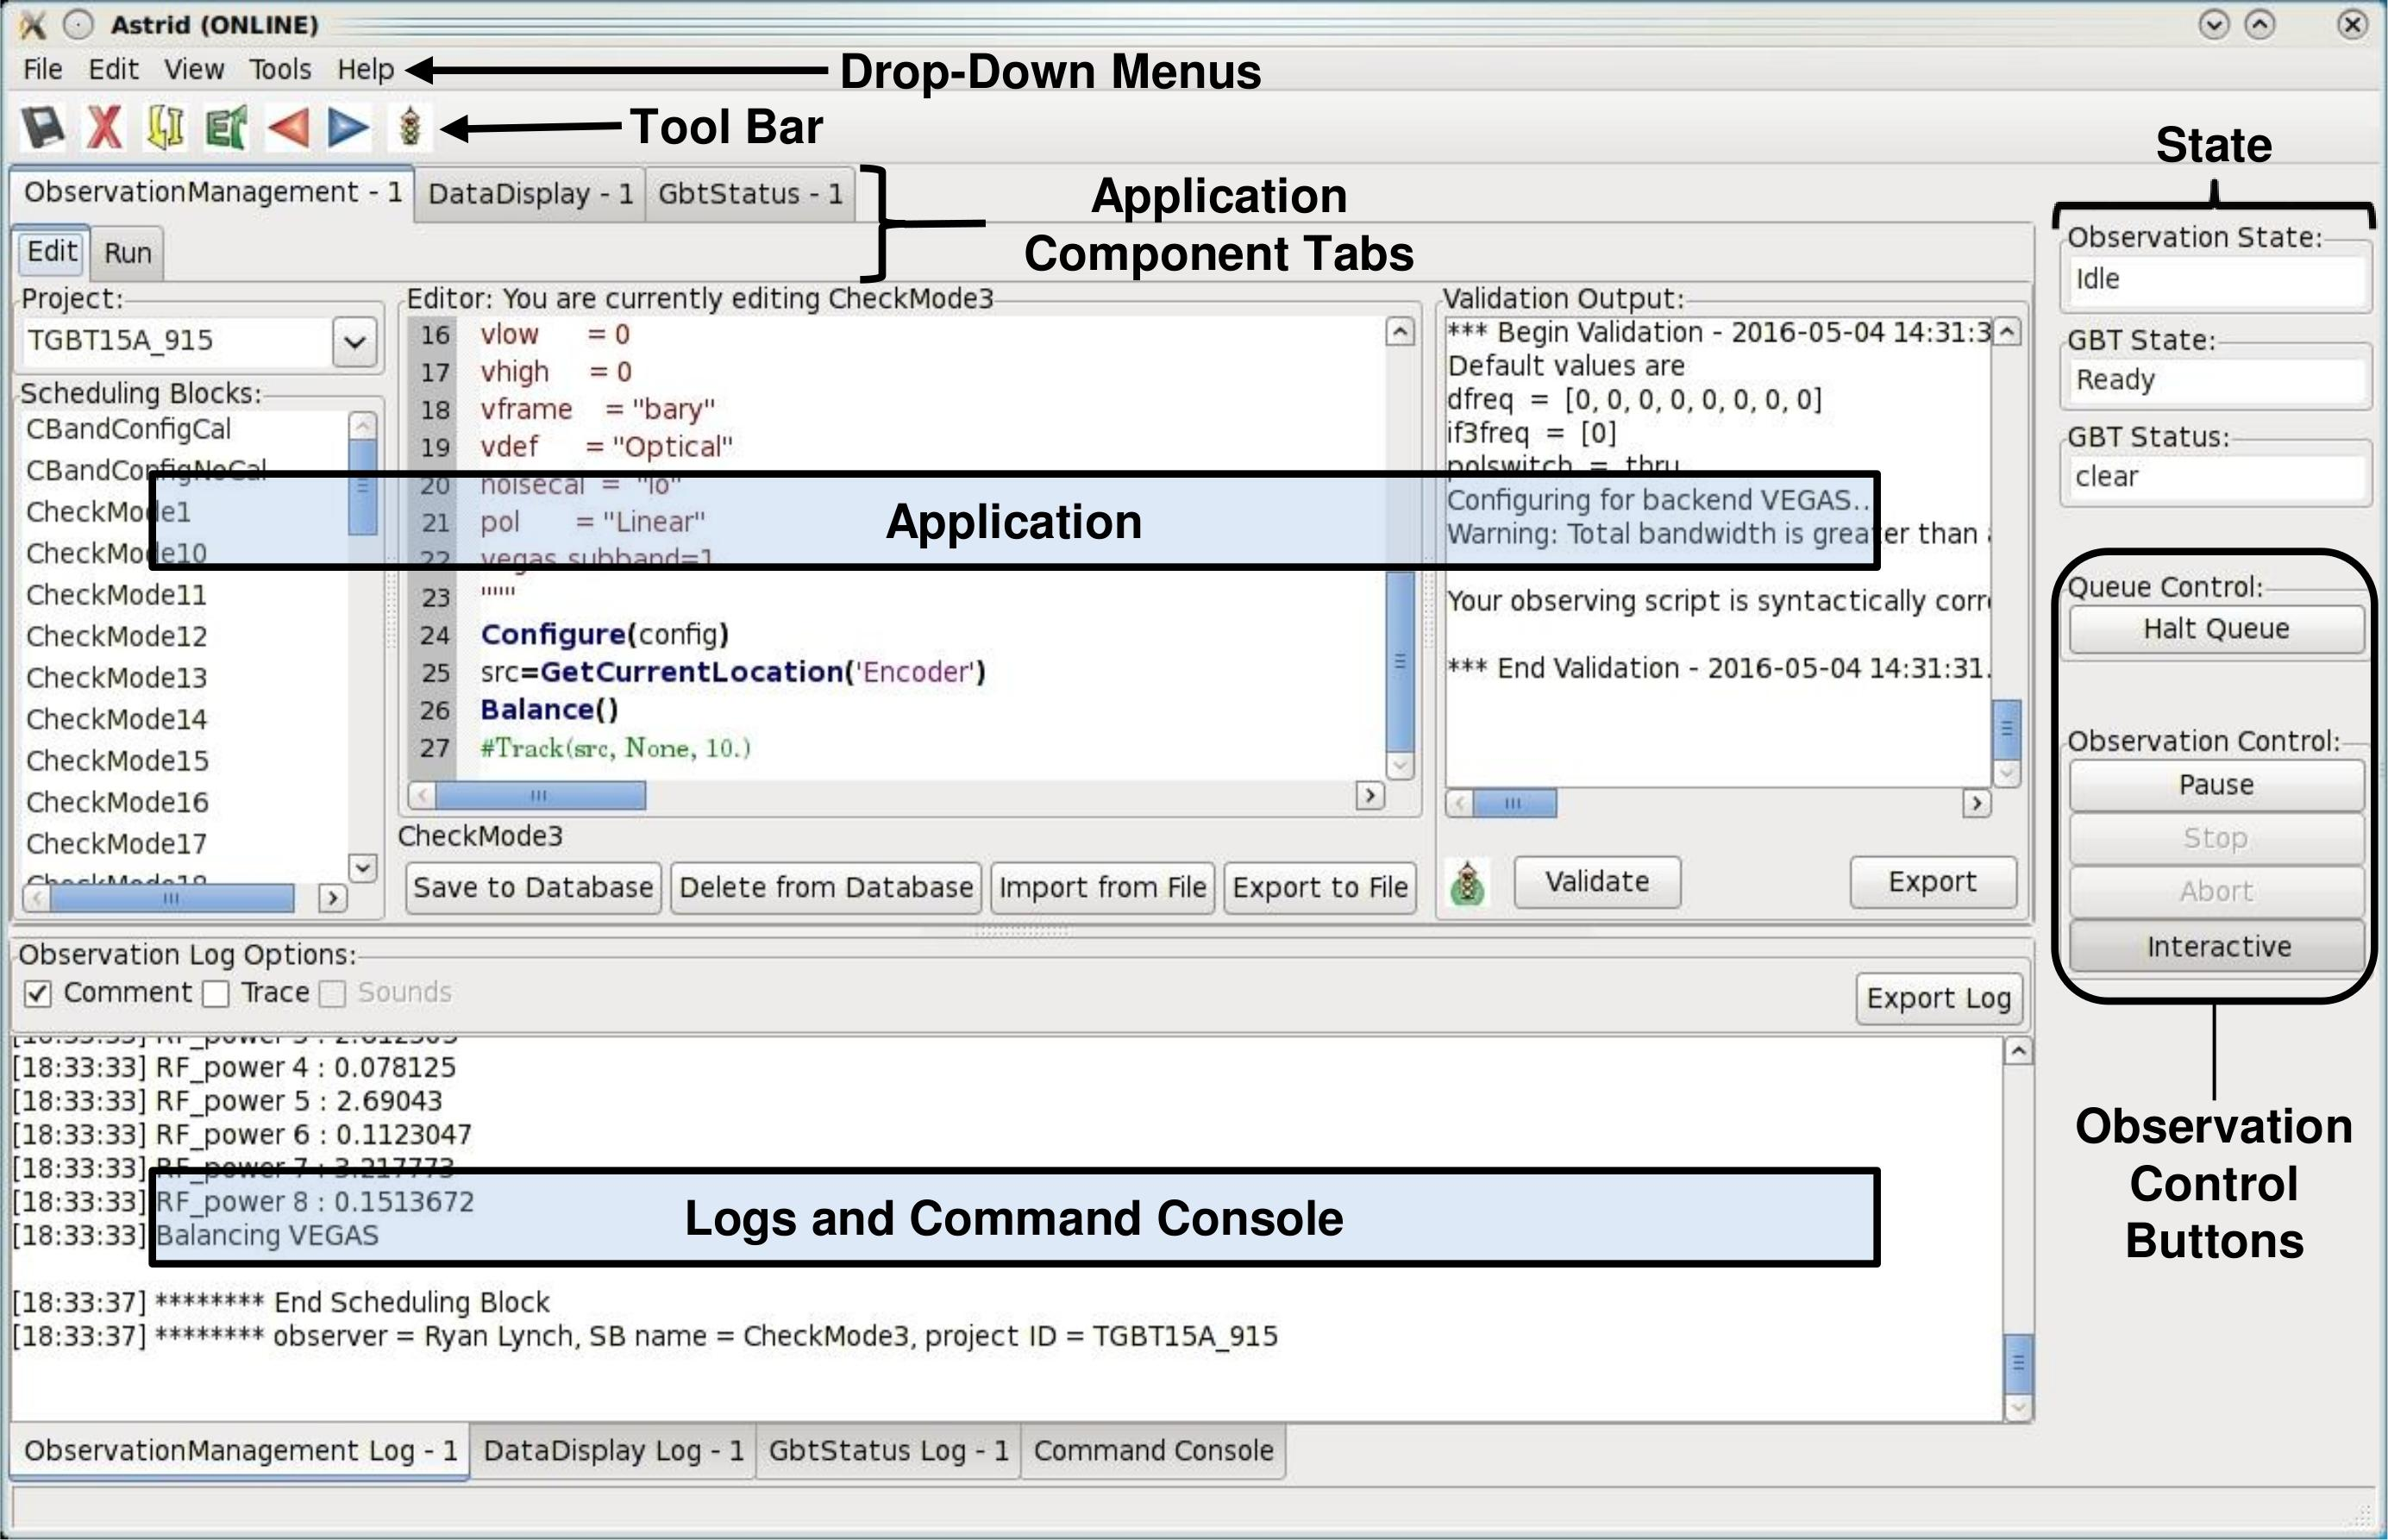
\includegraphics[width=\linewidth]{Astrid_components.jpg}
\caption[Components of the Astrid GUI]
{The different components on the \gls{Astrid} \gls{GUI}.
\label{fig:astridcomposition} }
\end{center}
\end{figure}

\subsection{Resizing Astrid Display Areas}

It is possible to resize some of the display areas within \gls{Astrid}.  If 
you put the mouse over the bar separating two display areas you will
get a double-arrowed resize cursor.  If you then hold down the
left--mouse button you can use the mouse to move the border and resize
the display areas.

\subsection{Application}

This comprises the majority of the space within the \gls{Astrid} \gls{GUI}.  This 
shows the contents of the Application selected by the application component tabs.

\subsection{Application Component Tabs}

The application component tabs are located under the Drop-down menus and the Toolbar
The top level of tabs allow users to switch between the three main \gls{Astrid}
applications: Observation Management, Data Display, and GBT Status.  Below these
are a set of subtabs that vary for each application component tab.

\newpage

\subsection{Drop--down Menus}\label{sec:dropdownmenus}

In the top, left hand side of the \gls{Astrid} \gls{GUI} you will find the drop--down
menus.  The contents of the drop--down menus change according to which
Application is currently being displayed on the \gls{Astrid} \gls{GUI}.  We will
not discuss all of the options under the drop-down menus in this document
but we will provide some highlights.

\begin{description}[leftmargin=*]
\item[File]
\begin{itemize}[itemsep=0pt,leftmargin=*]
\item[-] {\bf New Window} Launch applications within the \gls{Astrid} \gls{GUI} or in an
independent \gls{GUI}.
\item[-] {\bf Close Window} Close the currently displayed application in the \gls{Astrid}
\gls{GUI}.
\item[-] {\bf Real Time Mode...} Change between the operational modes of \gls{Astrid} (see
\S~\ref{sec:astridmode}).
\end{itemize}

\item[Edit] Standard \dq{Windows} undo, redo, cut and paste options.

\item[View] Display or hide the Toolbar or view \gls{Astrid} in Full Screen mode.

\item[Tools] Only active for the Data Display Application.  You may use checkboxes to
select various tooltips such as {\tt info}, {\tt pan}, and {\tt zoom}.  You can also
change the \dq{Fitting Heuristics} used during the reduction of Pointing and Focus
Observations by selecting {\tt Options...} (see \S~\ref{sec:heuristics}).

\item[Help] Bring up documentation for some but not all Applications.

\end{description}


\subsection{Toolbar}

The Toolbar is located just under the Drop--down Menus near the top of the
\gls{Astrid} \gls{GUI}.  The contents of the Toolbar change depending on which
Application is being displayed in the \gls{Astrid} \gls{GUI}.  The Toolbar options
are a subset of commonly used options from the Drop--down Menus.  When you leave
the mouse situated over one of the Toolbar buttons for a few seconds a \dq{pop-up}
will appear that tells you what action the Toolbar button will invoke.

\subsection{Logs}
The Log Window is located in the lower portion of the \gls{Astrid} \gls{GUI}
underneath the Application display area.  Clicking on the log tabs at the very bottom
of the \gls{GUI} will display log information for the Observation Managament, Data Display,
or GBT Status applications.  Viewing a specific log will also change the application
window to display the matching application.

The contents of the Observation Management application Log may be saved to an external
file via the \astridbutton{Export Log} button.  Note that closing or restarting \gls{Astrid} will
clear the Observation Management Log.  If you wish to retrieve an unsaved observating log,
please contact your \gls{GBT} \dq{Friend}.

\subsection{Command Console}
The Command Console is a Python shell that imports the \dq{Configuration Tool} and
\dq{Balance} \glspl{API}.  Both \glspl{API} will only interact with the \gls{MC}
systems if the user has been granted security access and is operating \gls{Astrid}
from the \dq{Work online with control of the telescope} mode (see \S~\ref{sec:astridmode}).

Observers may find the Command Console useful as a stand alone Python Shell.  However,
the \dq{configuration tool} and \dq{Balance} \glspl{API} are only intended for use by
\gls{GBT} staff and expert users.  Note that internal \gls{Astrid} commands
such as those listed in Chapter~\ref{chap:scripts} are not available for use without
first importing all necessary \gls{Astrid} modules.

\newpage

\subsection{State}\label{sec:GBTstatusDescription}

Three indications of state are located in the upper right corner of the \gls{Astrid}
\gls{GUI}.

\begin{description}[leftmargin=*,itemsep=0pt]
\item[Observation State] indicates \textbf{\gls{Astrid}'s state}.\\
If \gls{Astrid} is not communicating with the \gls{MC} system (such as in its
\dq{offline} mode) then you will see \dq{Not Connected}.  If \gls{Astrid} is
communicating with the \gls{MC} system and there isn't an \gls{SB} being executed
then you will see \dq{Idle} and if an \gls{SB} is running (or has been paused)
then you will see \dq{SB Executing}(\dq{SB Paused}). 

\item[GBT State] indicates the \textbf{\gls{MC} system state}.\\
If the \gls{MC} system is not working properly you will see \dq{Not In Service}
or \dq{Not Connected.} \dq{Unknown} indicates that the \gls{MC} system is working
but does not know the state of any of the hardware devices.  You will see the state
be \dq{Ready} when the \gls{GBT} is not doing anything.  It will be \dq{Activating}
or \dq{Committed} when the \gls{GBT} is preparing to perform an observation, etc.
While taking data during a scan the state will be \dq{Running}.  At the end
of a scan you will see the state become \dq{Stopping.}  If the scan is ended
for any abnormal reason the state will be \dq{Aborting.}

\item[GBT Status] indicates the \textbf{error state of the \gls{MC} system}.\\
If the \gls{MC} system is not communicating properly with the hardware the status can
be \dq{Unknown} or \dq{Not Connected.}  If the status is \dq{Clear}, \dq{Info},
or \dq{Notice}  then there are no significant problems with the \gls{GBT}.
If \dq{Warning} then it is worth asking the Operator what the problem is, but
it may not affect observation quality.  If the status is \dq{Error} then there
is potentially something wrong that may need attention. If the status is
\dq{Fault} or \dq{Fatal} then something has definitely gone wrong with the
observations.
\end{description}


\subsection{Observation Control Buttons}

The Observation Control Buttons are located in the lower-right of the \gls{Astrid}
\gls{GUI}. These buttons give the observer control of the \gls{GBT} during the
execution of an \gls{SB} and have the following functions:

\begin{itemize}[leftmargin=\widthof{\astridfixedbutton{Halt Queue}{6em}}]
\item[\astridfixedbutton{Halt Queue}{6em}] If this button is not activated then the \glspl{SB} in the Run queue
will continue to be executed in order. If this button is activated it will finish the current
\gls{SB} but will not allow the next \gls{SB} in the Run Queue to execute until the button
is returned to its default \dq{off} state.
\item[\astridfixedbutton{Pause}{6em}] Stop the execution of the current \gls{SB} when the next line of
code is encountered.
\item[\astridfixedbutton{Stop}{6em}] Stop the current scan at the end of the next integration time.
This is a nice, gentle way to stop a scan.
\item[\astridfixedbutton{Abort}{6em}] Stop the current scan immediately.  This may lead to corrupted data.
\item[\astridfixedbutton{Interactive}{6em}] When selected, will cause \gls{Astrid} to automatically
answer any pop--up query.  \gls{Astrid} will always choose what it deems
to be the safest answer.  This is useful when you have to leave the 
control for an extended period of time (such as when you go to the
cafeteria to eat, etc.).
\end{itemize}

\newpage

%++++++++++++++++++++++++++++++++++++++++++++++++++++++++++++++++++++++++++++
\section{The Observation Management Tab}

The Observation Management Application consists of two sub--\glspl{GUI},  the
Edit Subtab and the Run Subtab (see Figures~\ref{fig:astridedit} 
and~\ref{fig:astridrun}).  In the Edit Subtab you can create, load, save,
and edit \glspl{SB}.  You can also Validate that the syntax is correct.
The Run Subtab is where you will execute \gls{GBT} observations.
 
\subsection{The Edit Subtab}\label{sec:editsubtab}

The Edit Subtab has five major areas: a list of Project Names, \glspl{SB}
that have been saved into the \gls{Astrid} database for that project, an
editor, a Validation area, and a log summarizing the observations. This is
shown in Figure~\ref{fig:astridedit}. Chapter~\ref{chap:scripts} covers the
contents and creation of \glspl{SB}.

\begin{figure}[!h]
\setlength{\abovecaptionskip}{0pt}
\begin{center}
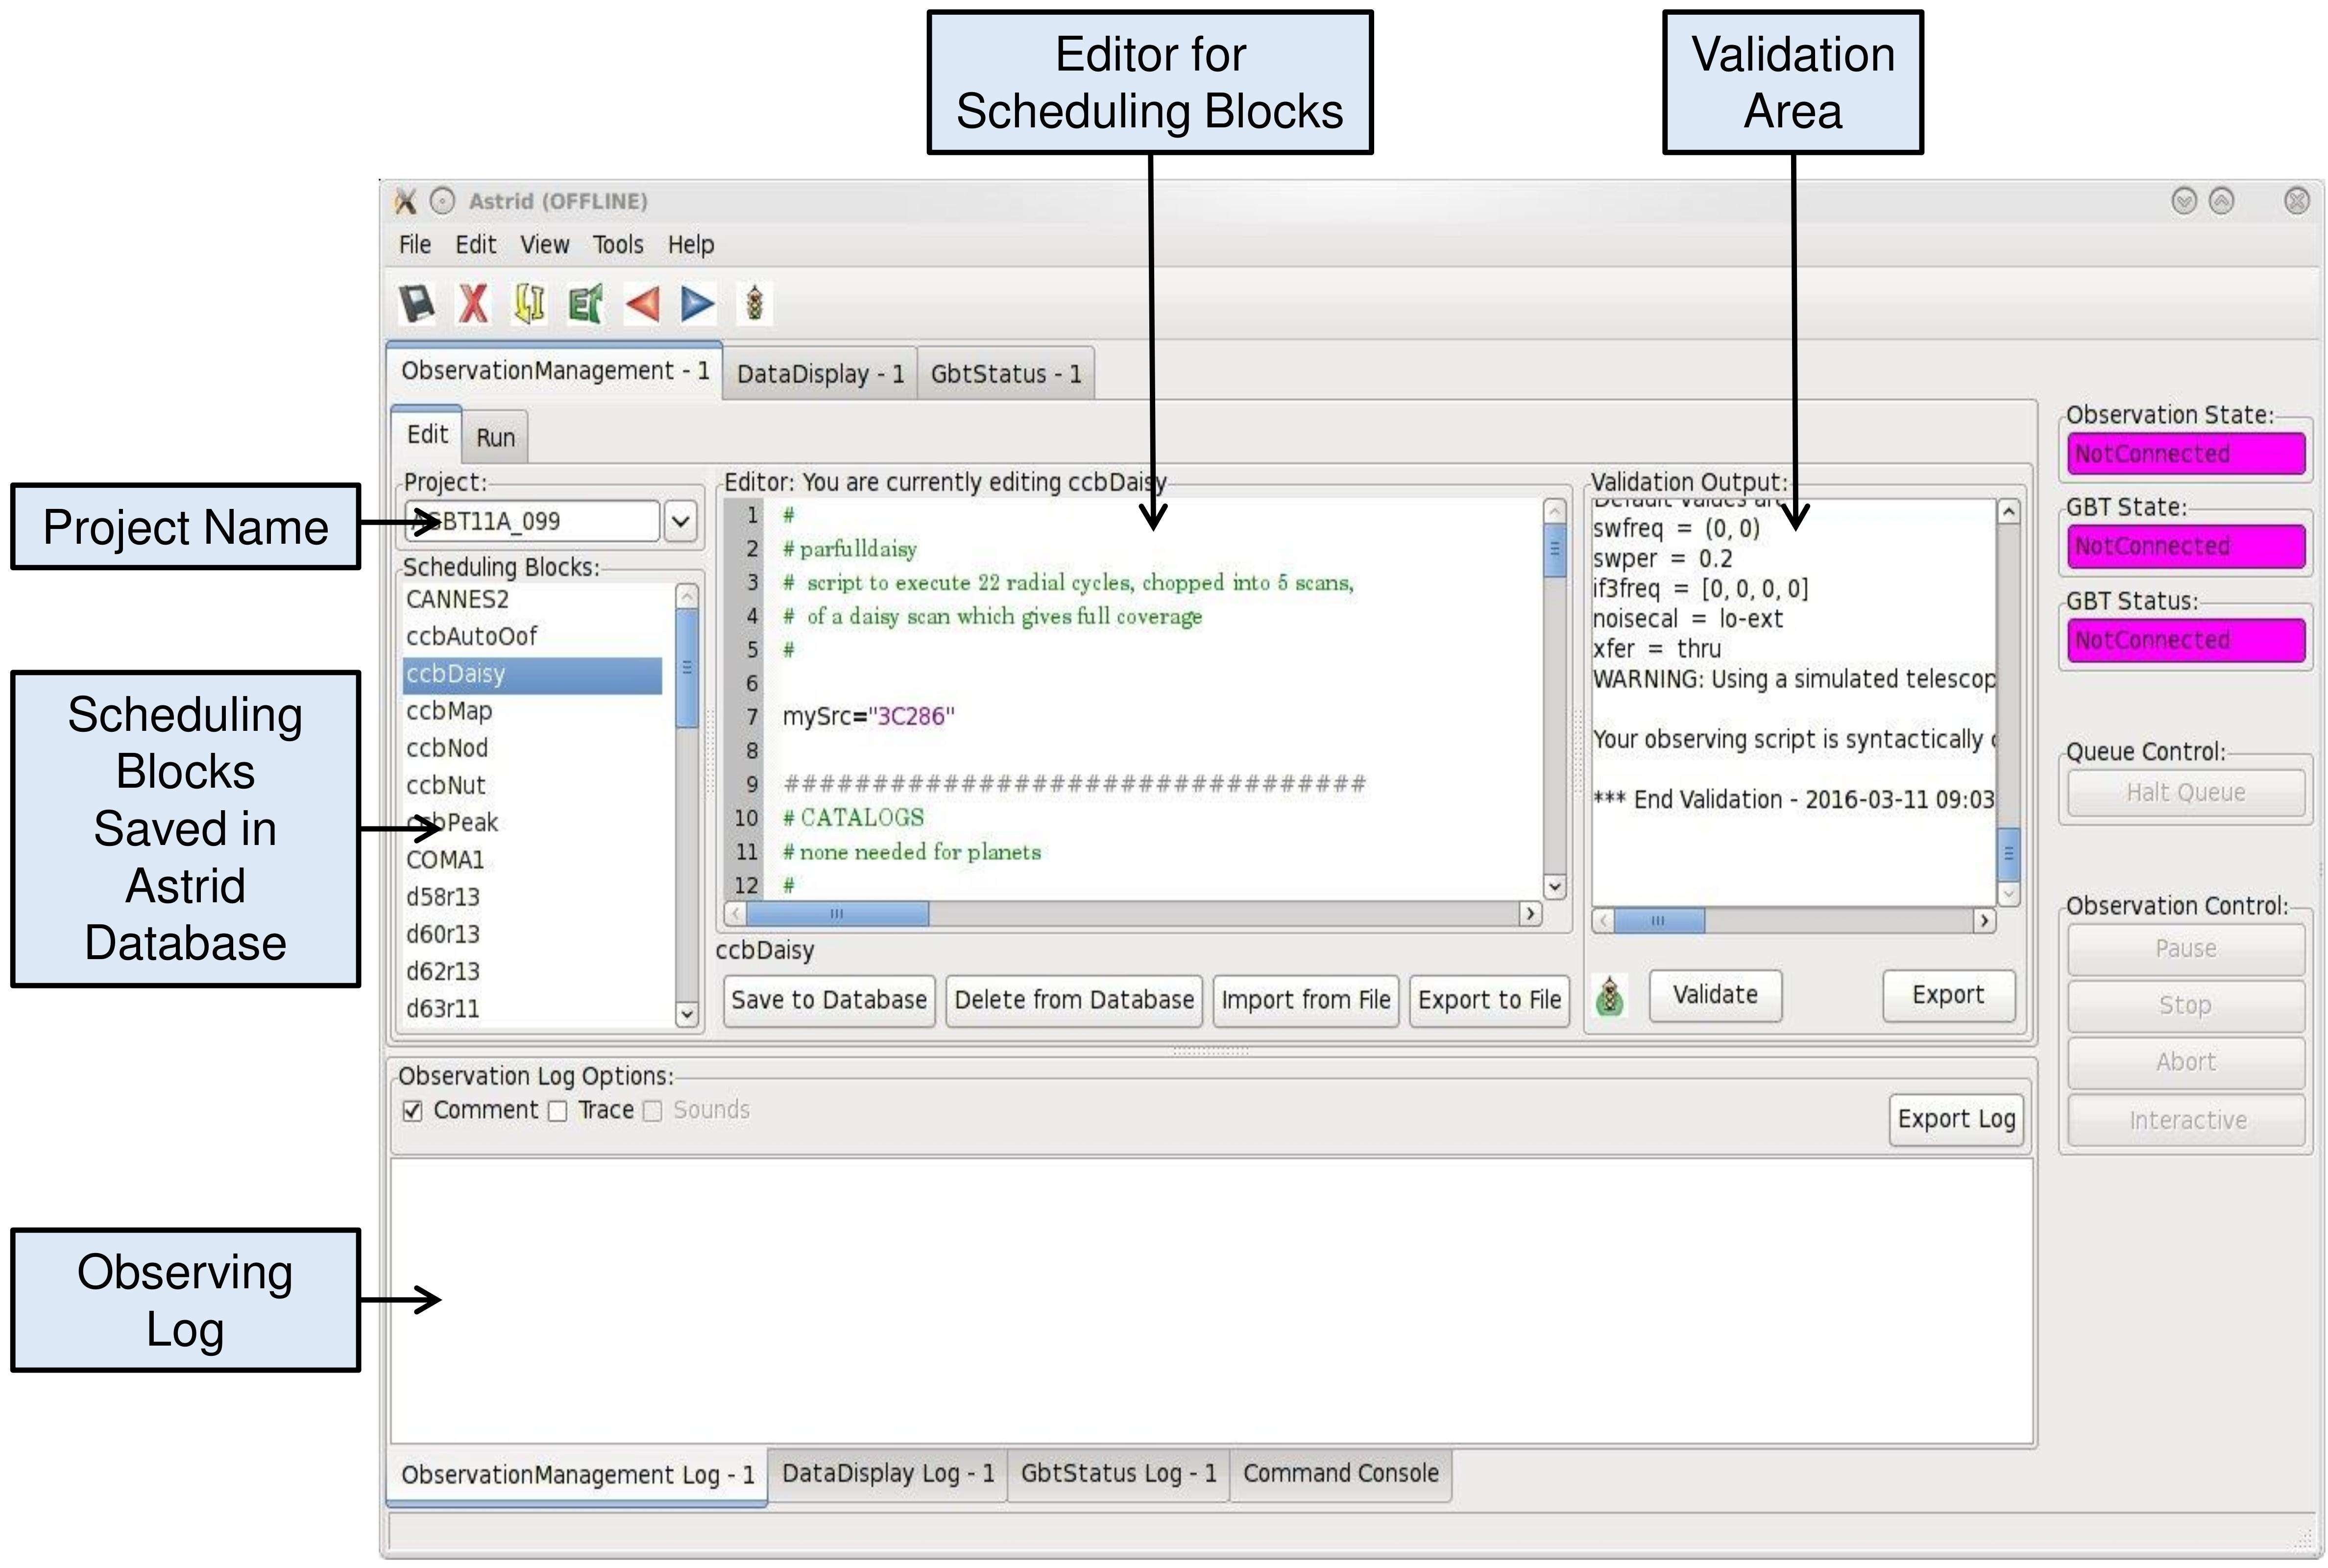
\includegraphics[width=0.90\linewidth]{AstridEditSubtab.jpg}
\caption[Astrid Observation Management/Edit Subtab]
{The \gls{Astrid} Observation Management/Edit Subtab. \label{fig:astridedit} }
\end{center}
\end{figure}

\subsubsection{Project Name and List of Scheduling Blocks}
\label{sec:projectID}
To access scheduling blocks associated with your project, you will need to
enter your Project Name in the \dq{project} window located in the upper left
part if the Edit Subtab.  Your Project Name is the code that your \gls{GBT}
proposal was given with the prefix \dq{AGBT}, e.g., AGBT16A\_001. To enter a
Project Name you may either type it in directly, or use the drop--down
arrows to navigate to your project through a project hierarchy as shown in
Figure~\ref{fig:projectHierarchy}

After doing this you will see in the window labeled \dq{Scheduling Blocks}
a list of \glspl{SB}, if any, that have been previously saved into the
\gls{Astrid} database. All of the saved \glspl{SB} for a given project will
show up in the \dq{Scheduling Blocks} section of the Edit Subtab.  If an \gls{SB}
has been Validated (i.e. it is syntactically correct) then it will appear
in bold--face type.  This means that it can be executed.  If the script
has been saved but is syntactically incorrect it will appear in  
lighter--faced type.

\newpage

\begin{figure}[!h]
\setlength{\abovecaptionskip}{0pt}\setlength{\belowcaptionskip}{0pt}
\begin{center}
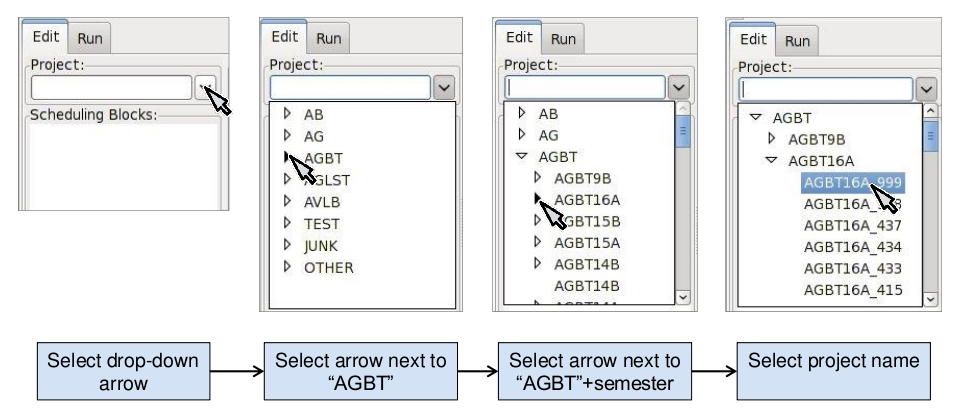
\includegraphics[width=0.9\linewidth]{projectHierarchy.jpg}
\caption[Selecting your project using the drop-down menu]
{Selecting your project using the drop-down menu. \label{fig:projectHierarchy} }
\end{center}
\end{figure}

\subsubsection{Editor}\label{sec:astridimport}

You can use the Editor to create or modify an \gls{SB} within \gls{Astrid}.  Standard
Windows functions like Ctrl--X (to cut selected text), Ctrl--C (to
copy selected text), and Crtl--V (to paste selected text) can be used within
the editor.  The editor lists the line number on the left hand side of the
window and marks Python code as follows:

\begin{itemize}[itemsep=0pt]
\item \textbf{\textcolor{pythonComments}{Green highlighted text}} - Commented characters
\item \textbf{Black highlighted text} - Standard Python commands/syntax
\item \textbf{\textcolor{pythonStrings}{Purple highlighted text}} - Strings
\item \textbf{\textcolor{pythonTripleStrings}{Magenta highlighted text}} - Triple quoted strings
(used in Python to enclose strings that span multiple lines)
\item \textbf{\textcolor{pythonKeywords}{Dark blue highlighted text}} - Python functions
\item \boldmath{$\ominus$}/\boldmath{$\oplus$} - Marks the start of an indented block of Python code
such as an {\bfseries{\textcolor{pythonKeywords}{if}}} statement or
{\bfseries{\textcolor{pythonKeywords}{for}}} loop.  Clicking on $\ominus$ will
collapse the indented code block and change the symbol to $\oplus$.  Likewise,
clicking on $\oplus$ will expand a previously collapsed code block.
\end{itemize}

\noindent The editor also has four operational buttons:

\begin{itemize}[itemsep=0pt,leftmargin=\widthof{\astridfixedbutton{blah}{10em} -}]

\item[\astridfixedbutton{Save to Database}{10em} -] This button will check the validation of the
current \gls{SB} and then save it to the \gls{Astrid} database.  A pop--up
window will notify you if the \gls{SB} did not pass Validation.  A second
pop-up window will allow you to set the name that the \gls{SB} will be saved
under in the \gls{Astrid} database.
\item[\astridfixedbutton{Delete from Database}{10em} -] This button will delete the currently selected
\gls{SB} from the \gls{Astrid} database.
\item[\astridfixedbutton{Import from File}{10em} -] This button will allow you to load an \gls{SB} from
a file on disk.
\item[\astridfixedbutton{Export to File}{10em} -] This button will allow you to save the edited \gls{SB}
displayed in the editor to a file on a disk.  This does not save the \gls{SB}
into the \gls{Astrid} database.
\end{itemize}

The first time you select either of the \astridbutton{Import from File} or
\astridbutton{Export to File} buttons you will have a pop--up window that
lets you select the default directory to use.  After selecting the default
directory you will get a second pop--up window that shows the contents of the
default directory so that you can select or set the disk file name to load
from or export to.

\newpage

\subsubsection{Adding and Editing Scheduling Blocks in the Database}

We will first describe how to add an \gls{SB} to the \dq{Scheduling Block} list
(i.e. database) and then we will describe how to manipulate and edit \glspl{SB}
in the list.

\begin{description}[leftmargin=*]

\item[Saving a Scheduling Block to the Database]\ \\
If you have already created an \gls{SB} outside of \gls{Astrid}, you should go to the
Edit Subtab in \gls{Astrid} and then use \astridbutton{Import from File} to load
your \gls{SB} into the Editor.  Otherwise you can just create your \gls{SB} in the
Editor.  To save the \gls{SB} into the \gls{Astrid} database you just need to hit
\astridbutton{Save to Database}.  This will run a validation check
(see \S~\ref{sec:validation}) on your \gls{SB} and then a pop--up window will appear
which allows you to specify the name which you would like to use in the list for your
\gls{SB}.

\item[Selecting a Scheduling Block]\ \\
If you perform a single click on any \gls{SB} in the \dq{Scheduling Block} list,
the contents of the selected \gls{SB} will appear in the Editor.  The selected \gls{SB}
will be highlighted with a blue background.

\item[Mouse--button Actions on the selected Scheduling Block]\ \\
If you perform a right mouse button click on the selected \gls{SB} a pop--up window
will appear that will let you rename, create a copy or save the \gls{SB} to the
\gls{Astrid} database.  You can also delete the \gls{SB} from the \gls{Astrid} database.
You may also rename the \gls{SB} if you perform a left mouse button double click
on the script name in the list.

\end{description}


\subsubsection{Validator}\label{sec:validation}

The Validation area is where you can check that the currently selected 
\gls{SB} is syntactically correct.  This does not check for run--time errors
and thus, does not guarantee that the script will do exactly what you want it to do.
For example, it can not check that you have the correct coordinates for your source.
You will also see error messages, notices and warnings from the Validation in this area.

The Validator will attempt to verify that you are using a legal configuration.
When run in \gls{Astrid}'s offline mode, the Validator can only compare your requested
configuration with a simulated \dq{ideal} model of the telescope hardware. To perform a
full configuration check against the true hardware state of the telescope (modelled by the
{\tt dev\_health.conf} file), you must be running \gls{Astrid} from the \dq{Work online
with control of the telescope} mode.

Before an \gls{SB} can be run within \gls{Astrid} it first must pass Validation.  To
Validate a script without saving it you can just hit \astridbutton{Validate}.
An \gls{SB} automatically undergoes a validation check when you hit
\astridbutton{Save to Database} in the editor.  Any messages, etc. from the
validation will appear in the \dq{Validation Output} test area. You can export
these messages to a file on disk by hitting \astridbutton{Export} in the
validation area.

The state of an \gls{SB}'s validation is shown by the stop--light. If the script has
never been validated or has been changed since the last validation the
stop--light will have the yellow light on.  If the \gls{SB} fails validation the
stop--light will turn red, while it will turn green if the \gls{SB} passes validation.

\noindent {\bf Note:} {\bfseries{\textcolor{pythonKeywords}{for}}} loops with many
repeats can take an extended amount of time to validate since the Validator will
go through each step in the loop. Also be careful of infinite loops in the
validation process.  Use of time functions such as
{\bfseries{\textcolor{pythonKeywords}{Now}}()} (see Chapter~\ref{chap:scripts})
always return \dq{None} in the validation.

\subsubsection{The Observing Log}

The observing log is always visible at the bottom of the Observation Management
Tab.  It shows information from the execution of \glspl{SB} in either of the
\gls{Astrid} online modes.  The observing log can be saved to a disk file
by hitting the \astridbutton{Export} button that is just above the top right corner of the
log display area.  Note that closing \gls{Astrid} will clear the observing log.
If you wish to retrieve unsaved observing log information, please contact your
\gls{GBT} \dq{friend}.


\newpage


\subsection{The Run Subtab}\label{sec:runsubtab}

The Run Subtab is shown in Figure~\ref{fig:astridrun}.  Here you will queue up
\glspl{SB} to perform the various observations that you desire to make. The Run
Subtab has five components.  Across the top of the Run Subtab you enter
information that will be put into the headers associated with the observations.
On the left is a list of \glspl{SB} that you can execute.  On the right are the
\dq{Run Queue} which holds \glspl{SB} that are to be executed in the future,
and the \dq{Session History} which shows which \glspl{SB} have previously been
executed.  At the bottom is the \dq{Observing Log}.

\begin{figure}[!h]
\begin{center}
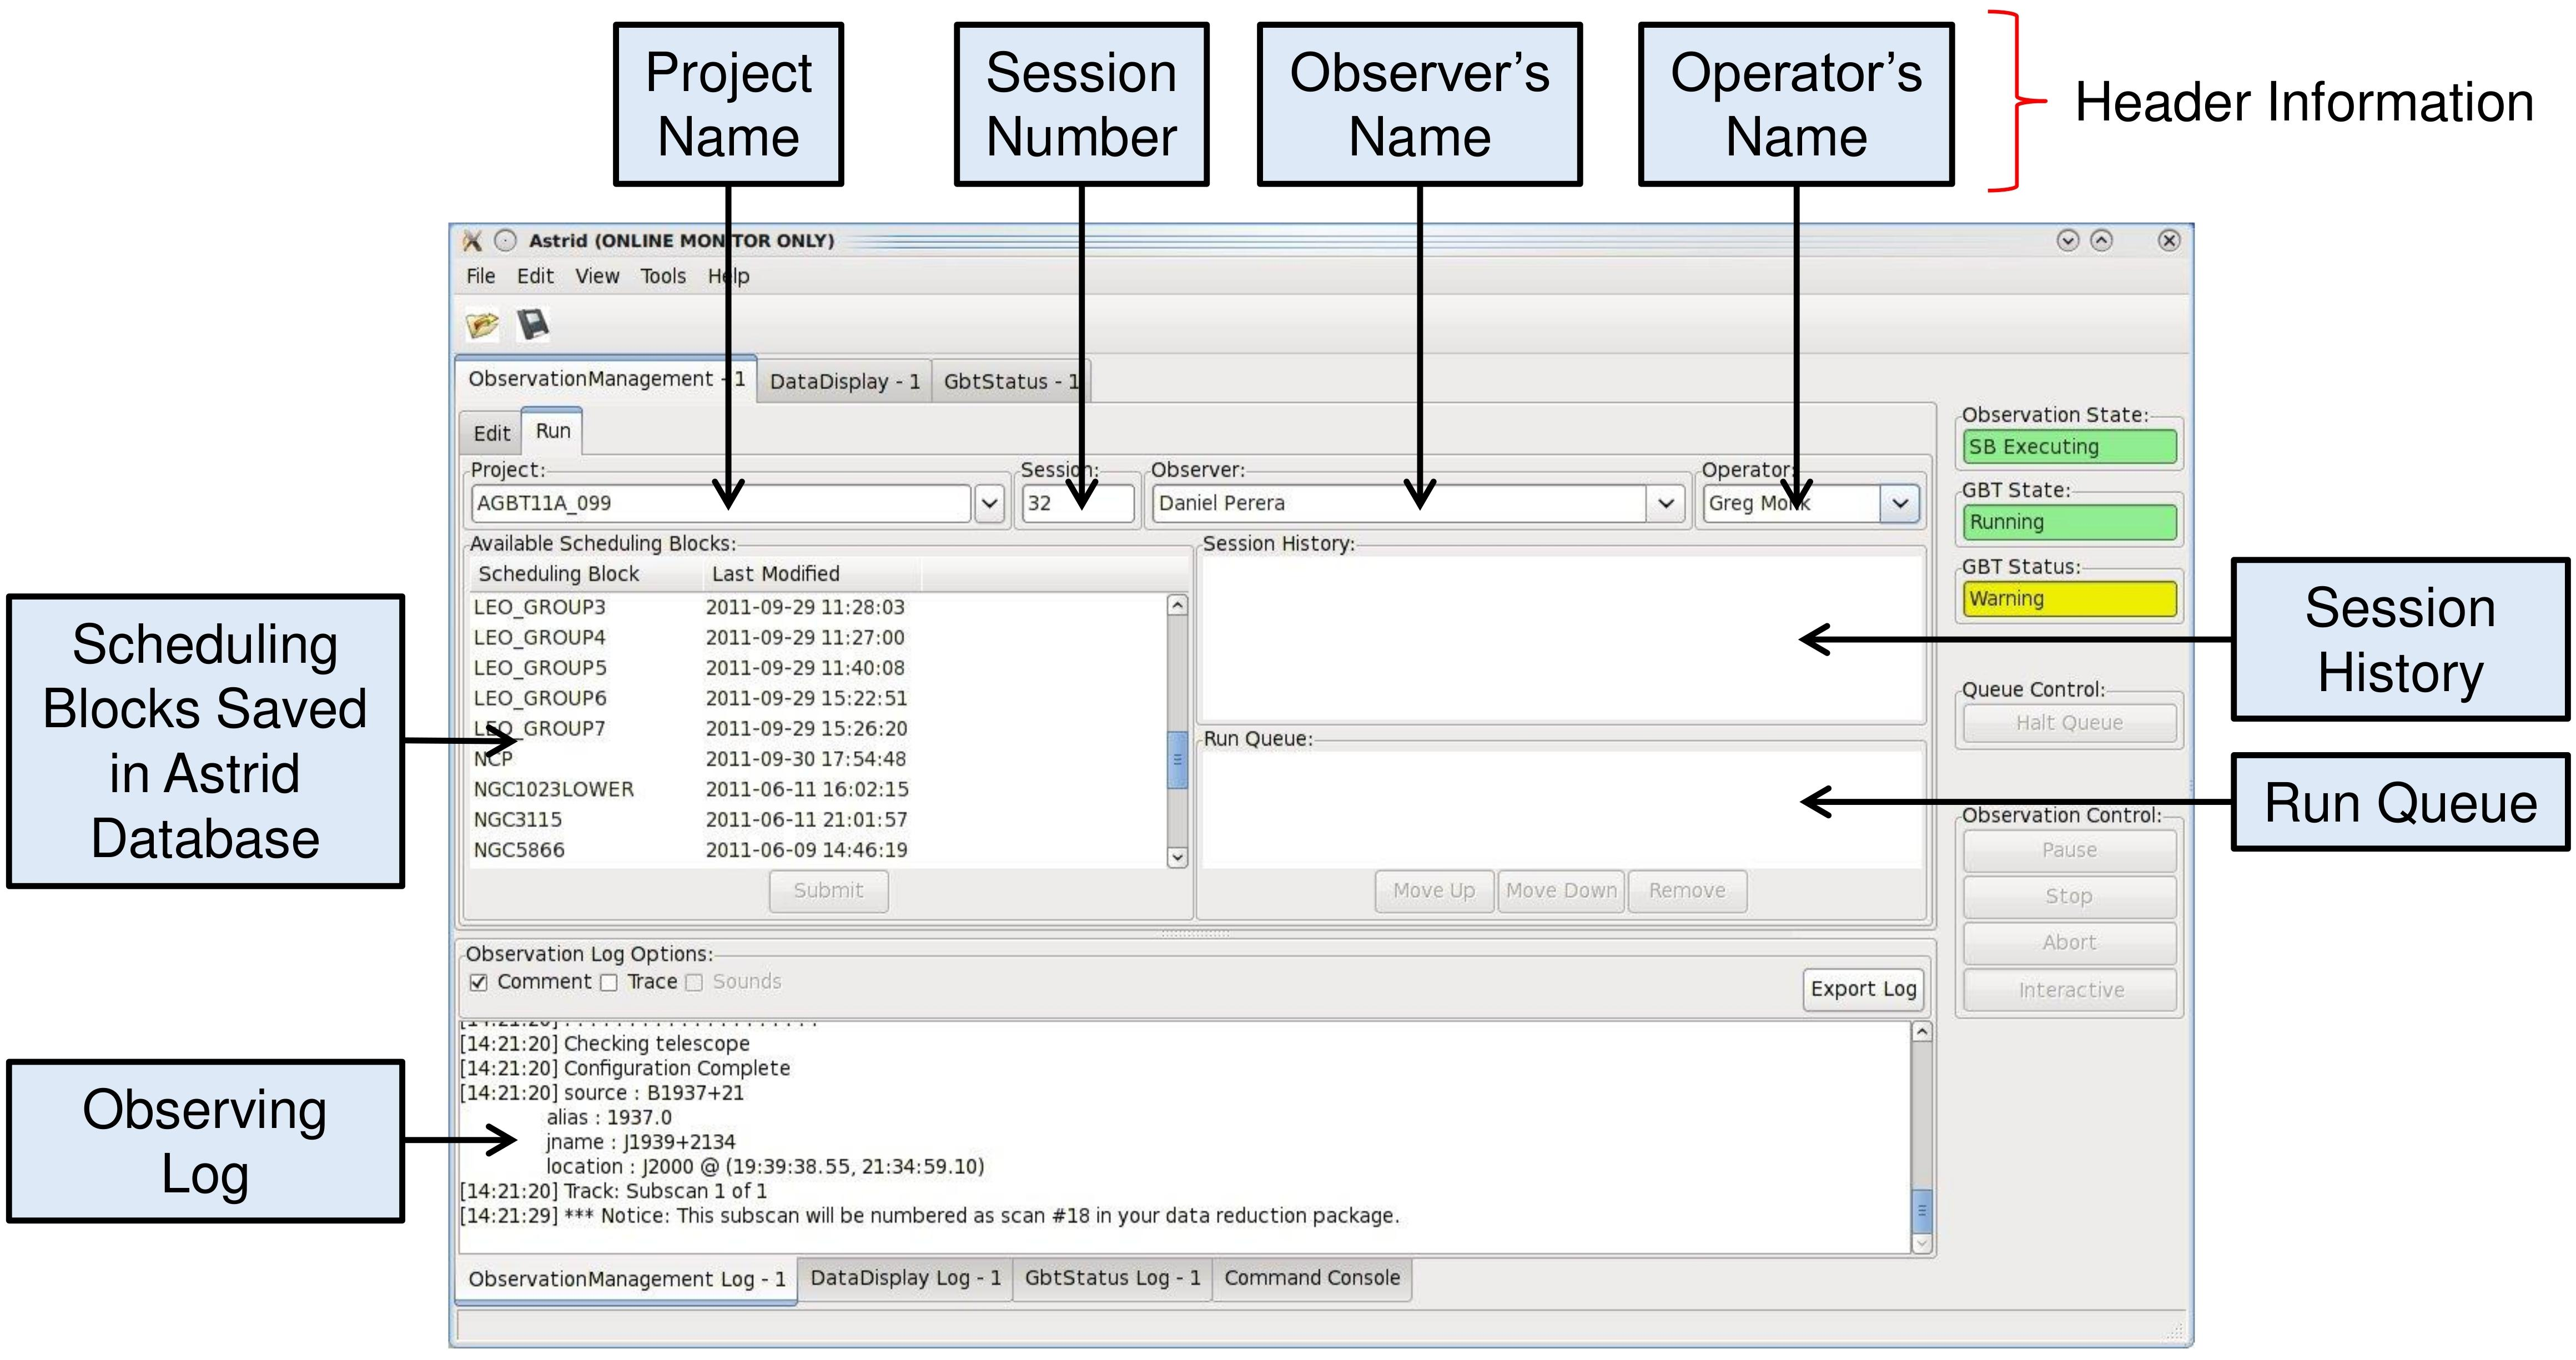
\includegraphics[width=\linewidth]{AstridRunSubtab.jpg}
\caption[Astrid Observation Management/Run Subtab]
{The \gls{Astrid} Observation Management/Run Subtab. \label{fig:astridrun} }
\end{center}
\end{figure}

\subsubsection{Header Information Area}

The following fields must have entries before an \gls{SB} can be executed:
\begin{description}[leftmargin=*]
\item[Project:] Just as in the Edit Subtab you use the drop--down menu to select
your Project Name. If your project is not listed, ask your \gls{GBT} \dq{friend} or the
telescope Operator to add it to the database.
\item[Session:] A session is a contiguous amount of time (a block of time) for which
the project is scheduled to be on the telescope.  Each time a project begins
observing for a new block of time it should have a new session number. The session
number is usually determined by \gls{Astrid} and automatically entered. However, there
are cases (such as \gls{Astrid} crashing) where the session number could become
incorrect.  You can type in the correct session number if needed. {\bf Note that a
\dq{Session} in \gls{Astrid} is equivalent to an \dq{observing period} in the lingo of the
\glsfirst{DSS}. \dq{Session} has a different meaning in the \gls{DSS}.}
\item[Observer's Name:] This is a drop--down list where you choose the observer's
name.  Only the \glspl{PI} on a project are guaranteed to have their name in this list.
If your name is not listed, ask your \gls{GBT} \dq{friend} or the telescope operator to
add it.
\item[Operator's Name:] This is a drop--down list from which you pick the current
operator's name at the beginning of your observations.
\end{description}

\newpage

\subsubsection{Submitting An SB to the Run Queue}

In order to execute an \gls{SB} you must:
\begin{enumerate}[label=\bfseries{Step \arabic*.},leftmargin=*,
labelindent=\parindent, itemsep=1pt]
\item Select the Observation Management Tab. 
\item Select the Run Subtab.  
\item Make sure that the header information fields all have entries.  
\item Select the \gls{SB} you wish to execute from the list of available \glspl{SB}.  
\item Hit the \astridbutton{Submit} button below the list of \glspl{SB}.
\end{enumerate}
Your \gls{SB} is then automatically then sent to the Run Queue.  Note that double-clicking
on an \gls{SB} is the same as selecting the \gls{SB} and then hitting \astridbutton{Submit}.

\subsubsection{The Run Queue and Session History}

When an \gls{SB} is submitted for execution it is first sent to the Run Queue.  This
contains a list of submitted \glspl{SB} that will be sequentially executed in the future.

When an \gls{SB} begins execution it is moved to the Session History list.  So the
Session History list contains the currently executing \gls{SB} on the first line and all
previously executed \glspl{SB} that have been run while the current instance of \gls{Astrid}
has been running on subsequent lines.

If there are not any \gls{SB} in the Run Queue when a new \gls{SB} is submitted
for execution it may appear that the \gls{SB} just shows up in the Session History.
However it has indeed gone through the Run Queue - albeit very quickly.

\subsubsection{The Observing Log}

The observing log is always visible at the bottom of the Observation Management
Tab.  It shows information from the execution of \glspl{SB}.  The observing log can be
saved to a disk file by hitting the \astridbutton{Export} button that is just above the top right
corner of the log display area.  Note that closing \gls{Astrid} will clear the observing log.
If you wish to retrieve unsaved observing log information, please contact your \gls{GBT}
\dq{friend}.

%++++++++++++++++++++++++++++++++++++++++++++++++++++++++++++++++++++++++++++
\section{The Data Display Tab}
 
The Data Display Tab provides a near--real time display of your \gls{GBT} data and
is discussed in Chapter~\ref{chap:datadisplay}.
\newpage
%++++++++++++++++++++++++++++++++++++++++++++++++++++++++++++++++++++++++++++
\section{The GbtStatus Tab}\label{sec:astridstatus}
 
The GbtStatus Tab displays various \gls{GBT} specific parameters, sampled values and 
computed values. Special care was taken to promote its use for remote 
observing.  An Example of how the \gls{GBT} Status Display appears in \gls{Astrid}
is shown in Figure~\ref{fig:astridstatusone} and~\ref{fig:astridstatustwo}.

\begin{figure}[!h] %general to scan/source
\begin{center}
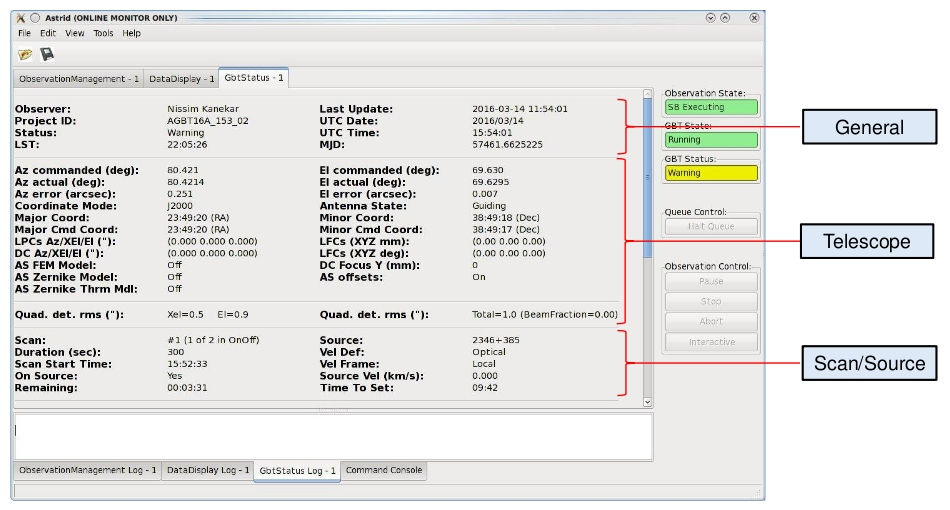
\includegraphics[width=\linewidth]{GBTstatus1.jpg}
\caption[Astrid Status Tab (top)]{The top portion of the \gls{Astrid} GbtStatus Tab.
To see the rest of the status screen you will need to use the scroll bar. 
\label{fig:astridstatusone} }
\end{center}
\end{figure}

The default status screen displays all of the currently supported items of 
the gbtstatus program grouped into various sections.  These are:

\subsection{General Status}
\begin{description}[leftmargin=*,itemsep=0pt]
\item[Observer:] The observer name.
\item[Project ID:] The data directory of the FITS files.  This is your Project Name
with the session as a suffix.  For example, the Project ID for session 02 of AGBT16A\_001
would be AGBT16A\_001\_02 (See \S~\ref{sec:projectID}).
\item[Status:] The status of the \gls{GBT}.  See \S~\ref{sec:GBTstatusDescription}
\item[LST:] The \glsunset{LST}\glsfirst{LST} of the last update.
\item[Last Update:] The local time when the database was last updated.
\item[UTC Date:] The \glsfirst{UTC} date of the last update. 
\item[UTC Time:] The \glsunset{UTC}\gls{UTC} time of the last update.  
\item[MJD:] The \glsunset{MJD}\glsfirst{MJD} of the last update.
\end{description}

\newpage

\subsection{Telescope Status}
\begin{description}
\item[Az commanded:] The commanded azimuth position of the telescope in degrees.
\item[Az actual:] The actual azimuth position of the telescope in degrees.
\item[Az error:] The difference between the commanded and the actual azimuth 
position of the telescope in arc-seconds.  This value does not contain a 
$\cos\left( {\rm el} \right) $ correction.
\item[El commanded:] The commanded el position of the telescope in degrees.
\item[El actual:] The actual elevation position of the telescope in degrees.
\item[El error:] The difference between the commanded and the actual elevation 
position of the telescope in arc-seconds.
\item[Coordinate Mode:] The coordinate mode used to represent a particular
location on the sky. See \S~\ref{sec:location_objects}
\item[Major and Minor Coord:] The telescope position in the current Coordinate Mode.
\item[Major and Minor Cmd Coord:] The telescope position in the current commanded
Coordinate Mode.
\item[Antenna State:] If the antenna software is not running the state will be
\dq{Disconnected.} If the antenna software is running but with its control of the antenna
turned off then the state is \dq{Dormant.}  If the antenna is not moving then the state
will be \dq{Stopped.}  If the antenna is moving and data are being taken then the state is
\dq{Guiding} and if data are not being taken the state is \dq{Tracking.}  If the antenna is
moving to a new commanded position the state is \dq{Slewing.}
\item[LPCs Az/XEl/El:] The \gls{LPC} offsets in arc-seconds.
\item[DC Az/XEl/El:] The \gls{DC} values in arc-seconds.
The \gls{GBT} has temperature sensors attached at various points on the backup
structure and the feed-arm.  These are used in a dynamic model for how the
\gls{GBT} flexes with changing temperatures.  This model is used to correct for
pointing and focus changes that occur from this flexing.
\item[LFCs (XYZ mm):] The \glsunset{LFC}\glsfirstplural{LFC} for the offset focus
position in millimeters.  This value is determined from a Focus observation
(see Chapter~\ref{chap:scripts}).
\item[LFCs (XYZ deg):] The subreflector tilt offset in degrees.
\item[DC Focus Y (mm):] The \gls{DC} Y subreflector offset in millimeters.
\item[AS FEM Model:] The  state of the \gls{FEM} correction for the \glsfirst{AS}.
The \gls{FEM} predicts how the surface changes due to gravitional flexure versus the
elevation angle.
\item[AS Zernike Model:] The  state of the \gls{AS} Zernike model correction model.
The Zernike model is a set of Zernike polynomial coefficients determined from
Out--Of--Focus holography that improve the shape of the \gls{AS} versus the elevation
angle.
\item[AS Zernike Thrm Model:] The  state of the \gls{FEM} correction for the \gls{AS}.
The \gls{FEM} predicts how the surface changes due to thermal flexure.
\item[AS Offsets:] The  state of the \gls{AS} zero offsets. The zero offsets are the
default positions for the \gls{AS}.  This should always be \dq{On} if the \gls{AS} is being
used.
\item[Quad. det. rms:] The quadrant detector is used to detect and correct for
wind-induced pointing errors.  rms values in arc-seconds are reported in elevation
and cross--elevation.  Total rms is also given as a fraction of the beam.
\end{description}

\subsection{Scan and Source Status}
\begin{description}
\item[Scan:] A scan is a command within an \gls{SB} used to collect observational data.
The field here is derived from the scan number and \gls{PROCNAME}, \gls{PROCSIZE}
and \gls{PROCSEQN} keywords from the \gls{GO} FITS file. 
\item[Duration:] The scan length in seconds.
\item[Scan Start Time:] If scan has started it is the \gls{UTC} scan start time - if the
scan has not started, then it is the countdown until the start of scan. 
\item[On Source:] \dq{Yes} or displays a countdown until the antenna is on source.
\item[Remaining:] The time remaining in the scan.
\item[Source:] The source name.
\item[Vel  Def:] The velocity definition specifies which mathematical equation is used to
convert between frequency and velocity.  See Equations~\ref{eq:vradio},~\ref{eq:voptical},
and~\ref{eq:vrel}
\item[Vel Frame:] The velocity frame or inertial reference frame.  See the \dq{vframe}
keyword in \S~\ref{sec:keywords}
\item[Source Vel:] The source velocity (km\,s$^{-1}$).
\item[Time To Set:] The time till the current source sets. 
\end{description}
\ \newline

\begin{figure}[!h]
\begin{center}
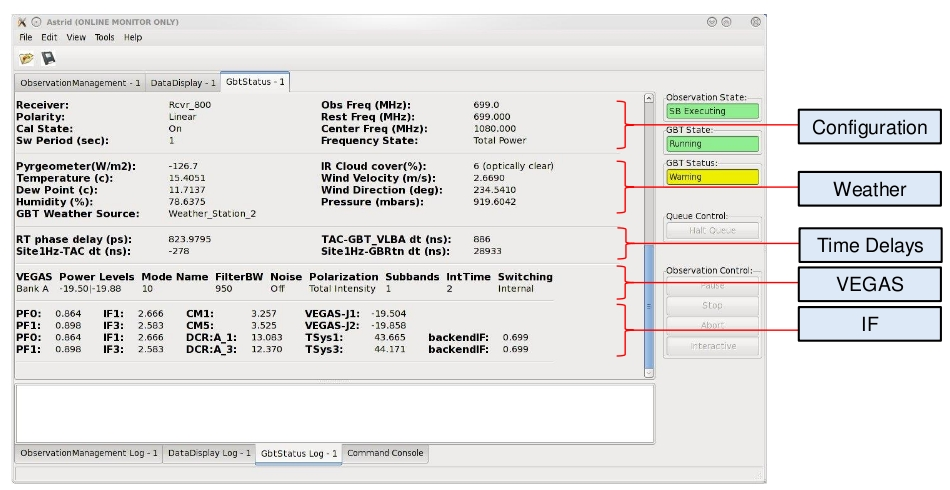
\includegraphics[width=\linewidth]{GBTstatus2.jpg}
\caption[Astrid Status Tab (bottom)]{The top portion of the \gls{Astrid} GbtStatus Tab.
To see the rest of the status screen you will need to use the scroll bar. 
\label{fig:astridstatustwo} }
\end{center}
\end{figure}
\newpage

\subsection{Configuration Status}
\begin{description}
\item[Receiver:] The receiver being used.
\item[Polarity:] The receiver polarity.
\item[Cal State:] \sq{ON} if the \gls{noiseDiode} is firing during the scan. 
\item[Sw Period:] The period in seconds over which the full switching cycle occurs.
This is determined by the user in their configuration (see \S~\ref{sec:config}).
\item[Obs Freq:] The observed spectral line frequency in the local frame (MHz).
\item[Rest Freq:] The spectral line frequency in the rest frame (MHz).
\item[Center Freq:] The center \gls{IF} frequency set by the \gls{LO} in MHz.  See
Appendix~\ref{appendix:spectralwindows} for further details.
\item[Frequency State:] The switching type.  Either \gls{tpower} or \gls{fsw}.
\end{description}

\subsection{Weather Status}

A real--time readout from one of the \gls{GBT} weather stations providing information on
temperature, pressure, humidity, dew point, wind direction and velocity. In addition,
the pyrgeometer measures the net near-IR irradiance of the sky to give an approximate
indication of cloud cover.

\subsection{Time Delay Status}
\begin{description}
\item[RT phase delay:] This is the time delay between the timing center in the \gls{GBT}
equipment room and the \gls{GBT} receiver room, in picoseconds, modulo 2000~ps.  It is measured
by comparing the phase of the 500~MHz reference signal  sent to the receiver room with a
copy of the signal returned to the  timing center.
\item[Site1Hz-TAC dt:] Time difference between the Site1Hz (a one pulse per second signal
that is locked to the hydrogen maser time standard) and a pulse from the GPS receiver
(\dq{TAC})
\item[TAC-GBT\_VLBA dt:] Time difference between the GPS receiver and the \gls{VLBA} back end
timing module.
\item[Site1Hz-GBTRtn dt:] Time delay between the Site 1Hz and a copy of the 1 Hz returned
from \gls{GBT} receiver room.  It is twice the delay of the fiber cables. The value is about
28933~ns which means the time delay between the equipment room the the receiver room is
about 14466~ns.
\end{description}

\subsection{VEGAS Status}
\begin{description}
\item[VEGAS:] The \gls{VEGAS} Bank (spectrometer with letter designation $A \rightarrow H$)
selected in the scan coordinator.
\item[Power Levels:] The power levels at the inputs to the \gls{VEGAS} \gls{ADC} cards.
There are two \glspl{ADC} per bank, one for each polarization. The \gls{VEGAS} balance
\gls{API} sets these values to approximately -20dBm by default.
\item[Mode Name:] Each \gls{VEGAS} Bank can be configured in one of 29 modes (see
Table~\ref{tab:vegas_modes}).
\item[FilterBW:] The bandwidth (MHz) of the digital filter implemented in the
\glsunset{FPGA}\glsfirst{FPGA}.  Note that these values do not correspond to the
bandwidths listed in Table~\ref{tab:vegas_modes}.
\item[Noise:] The state of the noise source which can be either \dq{On} or \dq{Off}.
\item[Polarization:] Users may specify which spectral product to record (See the \dq{vegas.vpol}
keyword in \S~\ref{sec:keywords}).  vegas.vpol=\dq{self} records \dq{Total Intensity} products,
\dq{cross} records \dq{Full Stokes} parameters, \dq{self1} records the polarization inputs
from the first \gls{ADC} only, and \dq{self2} records the polarization inputs from the second
\gls{ADC} only.
\item[Subbands:] Each \gls{VEGAS} bank can select between single (subbands=1) and multiple
(subbands=8) spectral windows when using VEGAS modes with a 23.44~MHz bandwidth.  
\item[IntTime:] The \gls{VEGAS} integration (dump) time in seconds.
\item[Switching:] Determines whether switching is controlled by \gls{VEGAS} (\dq{Internal}) or
another source (\dq{External}).

\end{description}

\subsection{IF Status}

The \gls{IFpath} in use are always displayed in the last section of the \gls{GBT}
status screen.  An example screen is shown in Figure~\ref{fig:astridstatustwo}.
Each line represents the \gls{IFpath} for a single polarization path from the 
\gls{IFRack} to the backend.  Each line contains only the devices in use for the 
listed path. A path may include a subset of the devices and values listed 
below.

\begin{description}[leftmargin=*]
\item[{\bf IF}\#:] The \# displayed is the number corresponding to the \gls{IFRack} 
switch in use. The value displayed is the \gls{RF} power in Volts detected by the 
\gls{IFRack}. 
\item[{\bf CM}\#:] The \# displayed is the number corresponding to the Converter 
Module in use. The value displayed is the \gls{RF} power in Volts coming out of the 
Converter Module after the \gls{LOtwo} and \gls{LOthree} mixers and before the Converter
Module filters. 
\item[{\bf CF}\#:] The \# displayed is the number corresponding to the Analog 
Filter in use. The value displayed is the \gls{RF} power in Volts coming out of the 
\gls{AFRack} after all filters have been applied (used with 100~MHz Converters).
\item[{\bf SG}\#:] The \# displayed is the number corresponding to the Analog 
Filter in use. The value displayed is the \gls{RF} power in Volts coming out of the 
\gls{AFRack} after all filters have been applied (used with 1.6~GHz Samplers).
\item[{\bf VEGAS-J}\#:] The \# displayed is the number corresponding to the port 
of \gls{VEGAS} in use. The value displayed is the power level in dBFS. For best
performance, it should be approximately -20 dBFS.
\item[{\bf Radar-Port}\#:] The \# displayed is the number corresponding to the port
of the Radar in use.
\item[{\bf DCR-Port}\#:] The \# displayed is the bank and number corresponding to 
the port of the \gls{DCR} in use. The value displayed is the total power in raw
counts. 
\item[{\bf TSys}\#:] The \# displayed is the number corresponding \gls{DCR} port
in use. The value displayed is the system temperature as reported by the \gls{DCR}
(should be considered a loose approximation).
\item[{\bf backendIF}:] The value displayed is the frequency of the Doppler track 
rest frequency as seen by the backend, in GHz.
\end{description}

%++++++++++++++++++++++++++++++++++++++++++++++++++++++++++++++++++++++++++++

%++++++++++++++++++++++++++++++++++++++++++++++++++++++++++++++++++++++++++++
%\section{The Command Entry Area}
 
%This is currently only used by expert pulsar observers.  If you wish
%to use this feature of Astrid you should contact your scientific support
%person.

%++++++++++++++++++++++++++++++++++++++++++++++++++++++++++++++++++++++++++++
%\section{\txtseccolor{Loading An SB -- 1/2 day}}
 
%++++++++++++++++++++++++++++++++++++++++++++++++++++++++++++++++++++++++++++
%\section{\txtseccolor{Executing An SB -- 1/2 day}}
 
%++++++++++++++++++++++++++++++++++++++++++++++++++++++++++++++++++++++++++++
%\section{\txtseccolor{Trouble Shooting -- 1 day (if needed)}}
%
%nothing

